\documentclass{standalone}

\usepackage{tikz}

\usepackage{bm}

\usetikzlibrary{angles, quotes}

\newcommand{\abs}[1]{\left| #1 \right|}

\begin{document}

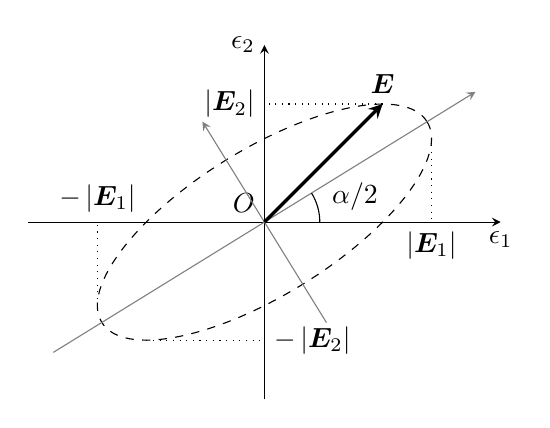
\begin{tikzpicture}[scale=1.5, >=stealth]
    \coordinate(O)at(0, 0);
    \coordinate(x)at(2, 0);
    \coordinate(a)at(31.68:2.5);
    \draw[->](-2, 0)--(x)node[below]{$\epsilon_1$};
    \draw[->](0, -1.5)--(0, 1.5)node[left]{$\epsilon_2$};
    \node[above left]at(O){$O$};
    \draw[dashed, rotate=31.68](O)ellipse[x radius=1.618, y radius=.618];
    \draw[->, gray, rotate=31.68](-2.1, 0)--(2.1, 0);
    \draw[->, gray, rotate=31.68](0, -1)--(0, 1);
    \draw[dotted](1.414, .707)--(1.414, 0)node[below]{$\abs{\bm E_1}$};
    \draw[dotted](-1.414, -.707)--(-1.414, 0)node[above]{$-\abs{\bm E_1}$};
    \draw[dotted](1, 1)--(0, 1)node[left]{$\abs{\bm E_2}$};
    \draw[dotted](-1, -1)--(0, -1)node[right]{$-\abs{\bm E_2}$};
    \draw[very thick, ->](0, 0)--(1, 1)node[above]{$\bm E$};
    \pic[draw, angle radius=20, angle eccentricity=1.7, "$\alpha/2$"]{angle=x--O--a};
\end{tikzpicture}

\end{document}